\chapter{Resultados y discusiones}
\lipsum[1]
\begin{table}[h!]
	\begin{center}
		\caption{Uso de split y color de celdas.}
		\label{tab:table1}
		\begin{tabular}{l|p{3cm}|r}
			
			\textbf{Value 1} & \textbf{Value 2} & \textbf{Value 3}\\
			$\alpha$ & $\beta$ & $\gamma$ \\
			\hline
			
			\multicolumn{2}{c|}{\cellcolor[gray]{.9}} & a\\
			\multicolumn{2}{c|}{\multirow{-2}{*}{\cellcolor[gray]{.9}1234}} & b\\
			\hline
			3 & \centering 23.113231 & c\\
			4 & 25.113231 & d\\
		\end{tabular}
	\end{center}
\end{table}

\lipsum[1]

\begin{figure}[H]
	\centering
	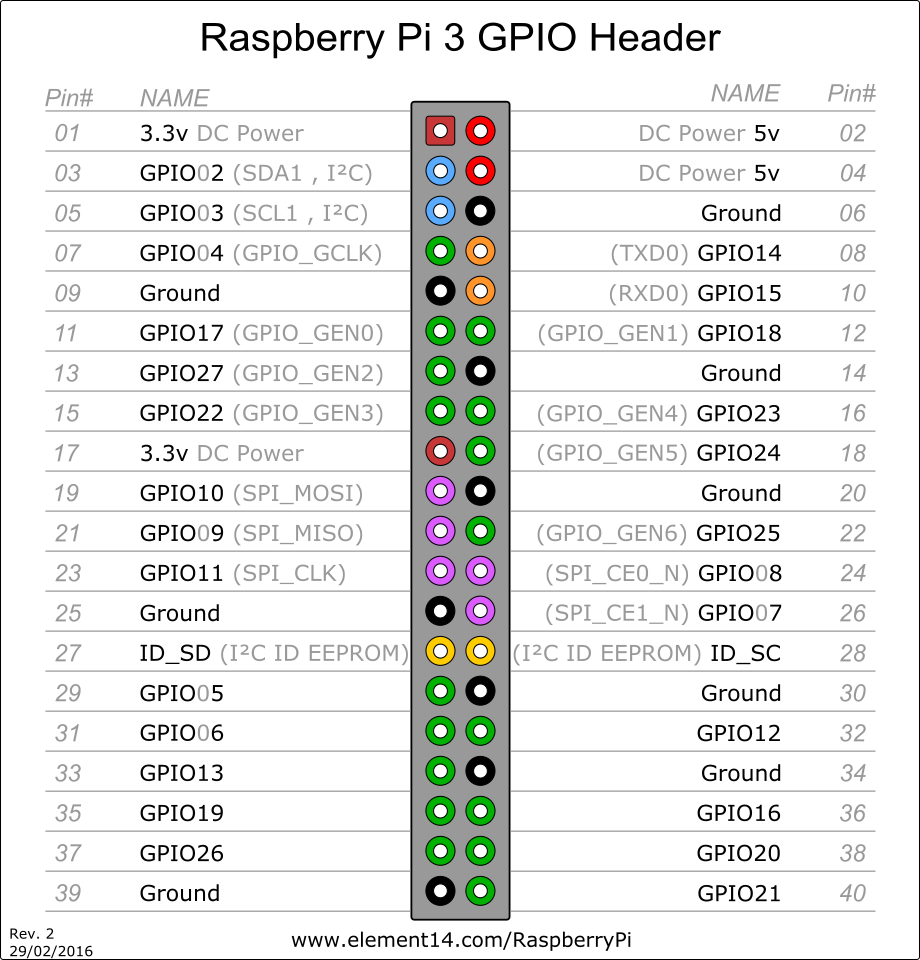
\includegraphics[width=0.7\textwidth]{figure/rpi3gpio.png}
	
	\caption{Raspberry Pi 3 Modelo B.  \\
		 Fuente:\href{https://www.w3schools.com/nodejs/img_raspberrypi3.png}{\itshape https://www.w3schools.com}}
	\label{gpio}
	
\end{figure}